\documentclass[11pt,a4paper]{article}
%PKG
\usepackage[utf8]{inputenc}
\usepackage[english]{babel}
\usepackage{amsmath}
\usepackage{amsfonts}
\usepackage{amssymb}
\usepackage{hyperref}
\usepackage{textcomp}
\usepackage{graphicx}
\usepackage{listings}
\usepackage{verbatim}

%PARAM
%Linux
%\graphicspath{{media/}}
%Windows
\graphicspath{{./media/}}

%FUNCTIONS
\newcommand{\centerFigure}[2]{
\begin{figure}[h]	
%Image: #1
\centering
\includegraphics[width=10cm]{#1}
\caption{#2}
\end{figure}
}

%DOCUMENT
\begin{document}
\pagestyle{headings}
\author{Axel Jeanne \and Monica Arias Rivera}
\title{Cooperative Supervised Mobile Manipulator}
\maketitle
\begin{abstract}
Robotic systems are growing in complexity and diversity due to the increasing challenges of the tasks
they are performing. As complexity increases, decoupling elements into smaller simpler parts is
regularly done. Following this decoupling trend, cooperative robotics grants an even 
larger change: using multiple robots to perform a single, yet complex, task.

This report present the work performed during the Supervised Mobile Manipulator (SMM) project.
The project consists in making a cooperative robotic system provide "smart" behaviour to
make the tele-operation easier to the user, while keeping effectiveness of the controlled robots 
unchanged.

For this project we used different hardware and software elements that we will introduce,
then we will present different cooperative behaviours and will expose their strengths and weaknesses; finally we will present the chosen system and expose its features and the results we obtained.
\end{abstract}
\clearpage

\tableofcontents

\clearpage
\section{Theoretical content}
\subsection{Advantages of cooperative system}
In most cases, the operator performing a task remotely only has a single point of view: the
one of the embedded camera. In multiple different systems, this can
lead to inconvenient situations where the operator is performing a task with a sub-optimal
vision of the situation.

One solution to this problem could be to add an animate vision system \cite{Ballard1991}
but this kind of solution vastly increases the complexity of the system since the whole vision system
has to be actuated. Another solution could be to increase the number of cameras on the robot.
This solution increases the robot payload and is actually not very convenient for the user
since more video streams now have to be monitored while performing the task. The solution we chose is to add an external robot to provide a "supervisor" vision of the acting robot. This solution adds many different  advantages:

\begin{enumerate}
\item The supervisor can provide vision from different angles while the action robot is static
\item The supervisor can scout ahead of the action robot to ensure safety
\item The supervisor behaviours can be automated to unload the operator's attention
\end{enumerate}


\subsection{Problem statement}
The Supervised Mobile Manipulator Project (SMM) goal is to develop a cooperative robotics
system which can be used in hazardous areas. It uses two platforms: 

\begin{itemize}
\item An action platform which perform the physical operation
\item A supervisor platform which keeps an overview of the situation
\end{itemize}

\centerFigure{teleopSystem.png}{The tele-operated robotic system}

To deliver a fully applicable solution, a GUI (Graphical User Interface) is provided in
order to see what the system is doing in real time.


\subsection{Tools used}
\subsubsection{Git}
To deliver a complete solution, a lot of software development was required. In order to keep
the code maintained and keep track of changes in code; we used \href{https://git-scm.com/}{git} as a version control system
 (VCS).

\subsubsection{ROS}
\href{http://www.ros.org}{ROS} stands for Robotic Operating System, although is not technically an OS. ROS is a middleware that provides an easy to use communication platform for different software and hardware elements. ROS was a very useful tool to implement cooperation in our system, particularly the network communication among robots.

\subsubsection{Gmapping}
The \href{http://wiki.ros.org/gmapping}{Gmapping} ROS package is an implementation of the Simultanous Localization and Mapping (SLAM) algorithm. It builds a grid map from a laser scan, and localizes the robot from odometry data and features extracted from the environment.

\subsubsection{Navigation Stack}
The \href{http://wiki.ros.org/navigation}{Navigation} ROS package enables a mobile robot to avoid obstacles in the environment (based on sensor readings), make a plan to reach a goal and produces appropriate velocities to get there. It accomplishes this through two separate implementations. 

First it builds a global costmap of the perceived environment, and builds a global path from the current position to the goal based on Djisktra's algorithm, obtaining the lowest cost path. This part is platform independent. 

Secondly it builds a local costmap, taking into account close obstacles and the global path, and sends the command velocities to the platform. The local planner is  platform dependant, and has to be tuned for optimal performance.

\subsubsection{Tum Ardrone}
The \href{http://wiki.ros.org/tum_ardrone}{Tum Ardrone} ROS package provides a PID controller for the AR Drone, coupled with a state estimation implementation with Extended Kalman Filter (EKF) and Parallel Tracking and Mapping (PTAM).

\subsubsection{Gazebo}
Gazebo is a well known and widely used simulator with a robust physics engine. 
Robot platforms like the TurtleBot and the AR Drone are already implemented, and new robots can be added using a SDF description. It also counts with different plugins  for robot, sensor, and environmental control. 

\subsubsection{Qt}
Qt is a well known GUI library. Is is used a large variety of applications from mobile phone interfaces to advanced customized programs. Qt is so popular that a module for ROS was
created called rqt (ROS Qt).


\subsection{Mobile base}

\begin{figure}[h]	
\centering
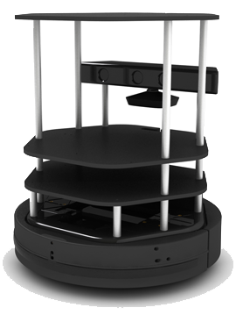
\includegraphics[height=5cm]{turtlebot.png}
\caption{The Turtlebot}
\end{figure}

The mobile base used is a TurtleBot. TurtleBot is a low-cost, personal robot kit with open-
source software
provided by different partners mostly for educational activities.
Our mobile base was equipped with an ASUS Xtion PRO, which uses an infrared sensor and adaptive depth detection technology. Having such information is very interesting for 
navigation
purposes since the relative distance to object is easily accessible.

\subsection{Quadrotor}
\centerFigure{arDroneGpsEdition.png}{AR Drone v2}

The quadrotor used is a Parrot\textcopyright AR Drone v2\texttrademark it is a 4 propellers
drone which has a ROS compatible driver. It is also equipped with two cameras: one in front
and another in the bottom. The bottom camera can be used for visual tracking and the drone
has an on-board tracking system, allowing a decent tracking without latency issues.

Additionally, some ROS libraries have been created to be compatible with the drone; we used
one of them called \href{"http://wiki.ros.org/tum_ardrone"}{"tum\_ardrone"} in parallel with
the driver package: \href{"https://github.com/AutonomyLab/ardrone_autonomy"}
{"ardrone\_autonomy"}.

\subsection{Cooperative behaviour}
As the two robots have to cooperate to perform their common goal, it was required to implement
cooperative behaviors on the system. During the conceptualization of the project we established different
cooperative behaviors that the system should be able to manage:

\begin{figure}[h]	
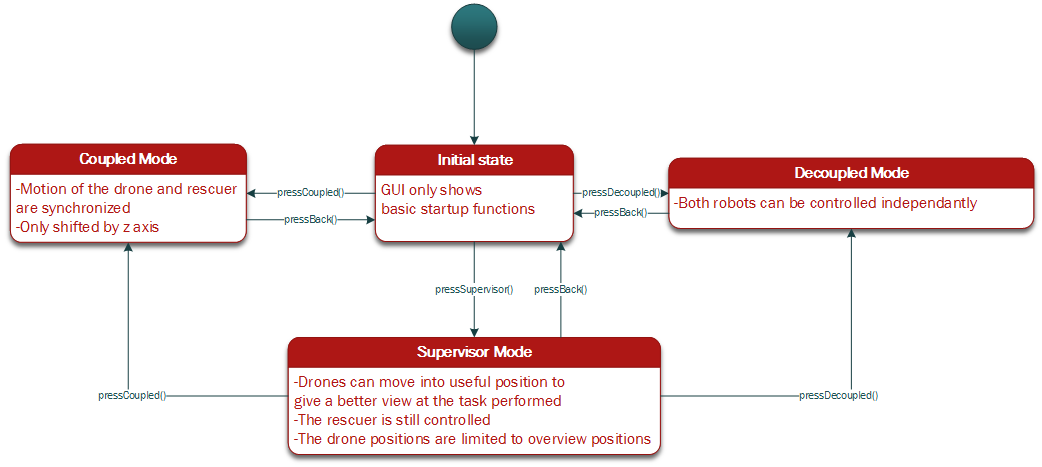
\includegraphics[height=7cm]{cooperativeModes.png}
\caption{Cooperative modes state map}
\end{figure}

\subsubsection{Default mode}
The default mode is the one in which the system start. No particular behavior is expected but the two
robots should establish connection and start exchanging their respective localization and status data.

\subsubsection{Coupled mode}
In this mode, the navigation of the two robots is linked, the mobile-base robot has asked the drone to 
rally on top of its position and the drone is tracking the mobile base underneath. From this point forward, if the mobile base moves, the drone remains on top and move along with it.

\subsubsection{Decoupled mode}
This mode is the same as default mode in terms of behaviour. The only difference is that the default mode
is not accessed any more after start-up. When the system enters the decoupled mode, the two robots movements
are decoupled and can be separately controlled, either by tele-operation or any other method.

\subsubsection{Assistance mode}
The assistance mode is a semi-operated mode. In this mode, the drone will adopt a set of pre-defined
positions around the mobile base. For instance in the case of navigation, the drone will move 
among a semi-circle (or full circle) around the mobile platform, allowing the 
operator to have better awareness of the situation.

\centerFigure{assistanceBehavior.png}{Map of the assistance behaviour}

Additional behaviours can be added into the assistance mode to be even more effective, for
instance adopting a lateral camera position while the robot is grasping an object. This would
allow the operator to have a real-time visual feedback on the action. Another behaviour
could be "forward scouting" allowing the drone to explore the area before engaging the 
mobile base.

\section{Work achieved}

\subsection{Individual Robot Capabilities}
In order to have smart behaviours, such that the operator does not need to be concerned with basic commands, some autonomous capabilities were implemented on both robotic platforms. Mainly autonomous navigation of unknown environments for the mobile base, and tracking, both a visual pattern and a given point, for the drone.

\subsubsection{Mobile Base}
Autonomous navigation of unknown environments was implemented with the Turtlebot.

The Gmapping ROS package was used to create a map of the environment as the Turtlebot travels through it, and to provide more robust localization within this created map. 

Navigating through the environment was done through the Navigation ROS package, allowing the robot to reach a defined goal, while avoiding obstacles. A special plugin was used to prioritize the path with the most clearance between obstacles. 



\subsubsection{Quadrotor}
The first achievement to make was to have visual tracking of the drone. For this task, we used 
the on-board control algorithm of the drone. This had many advantages: 
\begin{itemize}
\item The implementation was facilitated: activating the tracking on the drone can be done by 
setting a few parameters to different values. Then additional parameters can be tuned to
obtain a more or less robust tracking.

\item The delay in control is reduced: although we don't have full control on the control
loop, the delay between sending commands and command application is very short. According to
the average ping of the drone, the delay can vary from 50~ms to 3000~ms. In a control loop,
such fluctuations can make the system unstable.
\end{itemize}


\subsection{GUI programming}
Programming the GUI was facilitated by the rqt package. Setting up the interface was, however,
 a complicated task since the tutorial of rqt is not exactly finished and omitted crucial set-up details. The rqt package creates a ROS nodelet which allows access to
all the ROS useful features: subscriber, publisher, message types, etc.

Then this nodelet acts like a Qt blanc page, allowing us to program the GUI we want. It is 
important to note that the QWidgets and the ROS services run on a different thread, implying some limitations because a ROS Callback
\href{http://wiki.ros.org/rqt/Tutorials/Writing\%20a\%20C\%2B\%2B\%20Plugin}
{can't access a Qt element}.

Once the first test widget was operational, the development of the GUI could start: we had a 
first sketch of what we wanted so we developed the GUI along with the features we were
testing on the physical robot.
\centerFigure{guiSketch.png}{GUI version 0.1}

Then along with the functionalities, the GUI became more complex and diversified.
\centerFigure{guiV2.png}{GUI version 1.0}

In the final version of the GUI, an autopilot has been added, creating a new section in the 
GUI. This autopilot is based on the \verb!tum_ardrone! ROS package.
\centerFigure{guiV3.png}{GUI version 3.0}

\subsection{Robots interactions}


As the cooperation of robots could not be achieved before having total control over the two robots, 
we started programming the interactions toward the end of the project.

Then to have more robot interaction, it was necessary to make the two robots communicate.
The first interaction we wanted was to be able to perform a "rally on my position" procedure.
This was done by an event based approach in which the drone asks the Turtlebot for a point to go to. When the Turtlebot receives this request it broadcasts a new frame on top of it's position (where the drone should be at), and does the appropriate transformations to send the goto command to the drone's autopilot. The drone goes toward this point, and once it perceives the visual pattern it goes on to tracking the pattern, and the Turtlebot stops broadcasting this point.

\subsection{Simulator implementation}
In order to debug and test the cooperative behaviours without having to worry about the safety of the drone, we implemented a simulation of the whole system in Gazebo.

The Turtlebot has plenty of support in the community, and did not present any major difficulties to use it in the simulation. On the other hand, the AR Drone's simulator package (Tum Sim) was made originally for the Hydro version of ROS, one previous to the one we are using (Indigo). It was required to do some slight modifications to the SDF description files to make it compatible with our system.

Once we had each robot working separately on Gazebo, we had to be careful with topic and frame names when we launched them together. The namespace 'quadrotor' was used to launch the drone model and related nodes. By changing the topic names we had to modify the source code of the Tum Sim package again, since it was not possible to remap the sensor information topic names used to stabilize the drone.


\section{Result analysis and conclusions}
\subsection{Results analysis}
\subsubsection{Experiment 1}
The first test was to tele-operate the drone on top of the turtlebot, and let the on board control
manage the tracking.
%need image
%\centerImage{firstTest.png} 

The drone performing a "rally on me" operation.

The test was successful and no trouble arose during this phase. Indeed; tele-operating the drone is 
safe since we have total control over it's motion.
As expected, the on board controller managed to keep the drone stable while still tracking the mobile base 
movement. However we noted that this controller does not re-center the drone: if the drone has a static
error, the tracker won't compensate it: the drone will remain shifted.

\subsubsection{Experiment 2}
The second test was to perform the same operation but using the auto-pilot of the \verb!tum_ardrone!
package for rallying on top of the mobile base.

The experiment was not a total success, the auto-pilot rely a lot on the visual camera calibration to 
localize, and this lead to erratic behavior and static drifting.
The autopilot did get the drone on the desired position but then drift away periodically. This lead to the 
lost of track of the visual feature, leading to the interruption of the tracking.

We re-tried performing the experiment and again, the same stability issues happened. After a few tests we 
saw very different behaviors: sometime the auto-pilot would manage perfectly to go to position without any
drifting and sometime the drone would drift away dramatically. In order to minimize this problem, we 
automated the take off procedure to have the best possible camera calibration during take-off. This 
allowed to reduce the erratic behavior but didn't entirety solved the problem: erratic behavior can happen
especially of the front camera does not find enough visual keypoints.

\subsubsection{Experiment 3}
In order to verify the "rally on me" procedure, we implemented this setup into Gazebo simulator to test if
the position of the frames were correct and if the call to the frame transformation service was working.

The experiment in Gazebo went flawlessly, the drone stays perfectly stable and the frame attached to the 
mobile base is always align.

\subsection{Improvement and future work}
\subsubsection{Graphical user interface}
Improving the current GUI can be made by adding more dynamic elements into it. The current problem is
that it displays lots of information in a "raw" manner. The global design of the GUI could be revisited in
order to present all information  in a coherent and clear way.

\subsubsection{Cooperative behavior}
We have presented many different cooperative behavior for this system, however we only had time to 
implement one of them. It would be interesting now that the two robots are under control, to implement
different cooperative behaviors, test their stability and eventually keep the most robust and effective
one.

\subsubsection{Simulation}
As the simulator doesn't reproduce accurately the physical behavior of the drone, having a more detailed 
AR Drone model would help to test stability and control issues, without having to use the real physical 
system.

\section{Conclusion}


\bibliography{bib}
\bibliographystyle{abbrv}
\end{document}
